% FiLMVIB --- final internship presentation.  Build:  cd paper && pdflatex final.tex  (x2)
%
% Every value in this file is either (a) measured under our own evaluation protocol, with the
% source runs/*.json named in an adjacent comment, or (b) reported by a cited publication, with
% the arXiv identifier given in the row. Nothing here is estimated or extrapolated.
%
% Deliberately omitted for want of evidence: multi-seed statistics, the beta_kl sweep, the
% VIB-ingredient ablation, the data-scaling curve, and the video-substitution / MiniCPM-adapter
% results (trained but not yet evaluated at the time of writing; see the closing slide).
\documentclass[aspectratio=169,11pt]{beamer}
\usetheme{default}
\usecolortheme{seahorse}
\setbeamertemplate{navigation symbols}{}
\setbeamertemplate{footline}[frame number]
\setbeamertemplate{itemize items}[circle]
\setbeamertemplate{blocks}[rounded][shadow=false]
\setbeamerfont{frametitle}{size=\large,series=\bfseries}
\setbeamercolor{frametitle}{fg=blue!45!black}
\usepackage{tikz}
\usetikzlibrary{positioning,arrows.meta}
\usepackage{booktabs}
\usepackage{amsmath,amssymb}
\graphicspath{{figures/}}
\definecolor{frz}{RGB}{40,95,175}     % frozen
\definecolor{trn}{RGB}{210,120,20}    % trained
\newcommand{\figslot}[2]{\IfFileExists{figures/#1}%
  {\includegraphics[width=#2]{figures/#1}}%
  {\fbox{\parbox[c][2.6cm][c]{#2}{\centering\tiny\ttfamily\detokenize{figures/#1}}}}}
\newcommand{\frm}[1]{\IfFileExists{figures/#1}{\includegraphics[height=15mm]{figures/#1}}%
  {\fcolorbox{gray}{gray!12}{\parbox[c][14mm][c]{20mm}{\centering\tiny\ttfamily\detokenize{#1}}}}}
\newcommand{\frmrow}[1]{\frm{#1_1.jpg}\hspace{1pt}\frm{#1_2.jpg}\hspace{1pt}\frm{#1_3.jpg}}
\newcommand{\exrow}[5]{%
  \begin{tikzpicture}[font=\scriptsize,>={Latex[length=1.6mm]}]
    \node[draw=black!30,rounded corners=2pt,inner sep=1.5pt] (im) {\frmrow{#1}};
    \node[anchor=west,align=left,text width=58mm,inner sep=0pt] (c) at ([xshift=7mm]im.east)
      {#2\\[2pt]\emph{#3}};
    \draw[->,black!45] (im.east) -- (c.west);
    \node[draw=red!60!black,fill=red!8,rounded corners=2pt,inner sep=2.5pt,anchor=north west]
      (b) at ([yshift=-3pt]c.south west) {\color{red!72!black}base: #4 $\boldsymbol{\times}$};
    \node[draw=green!45!black,fill=green!12,rounded corners=2pt,inner sep=2.5pt,anchor=west]
      (o) at ([xshift=3mm]b.east) {\color{green!48!black}ours: #5 $\boldsymbol{\checkmark}$};
  \end{tikzpicture}}

\title{\textbf{Making Frozen Audio--Visual LLMs Listen}}
\subtitle{Audio grounding via tiny adapters, anchored preference optimization, and honest evaluation}
\author{Souleiman Sbai}
\institute{Research internship --- final presentation\\[2pt]
  \footnotesize Host lab: AIST CVRT \quad$\cdot$\quad Supervisor: Qiu Yue}
\date{\today}

\begin{document}

% ============ Title ============
{\setbeamertemplate{footline}{}
\begin{frame}
\titlepage
\vspace{-1.2em}
\begin{block}{}
\footnotesize Audio-visual LLMs frequently answer questions about sound using visual evidence. This work
introduces a parameter-efficient adapter that improves audio grounding in a \emph{frozen} backbone,
together with an evaluation protocol designed to test the claim rigorously.
\end{block}
\end{frame}}

% ================================================================
% ================================================================

\begin{frame}{What is an audio--visual LLM?}
\centering
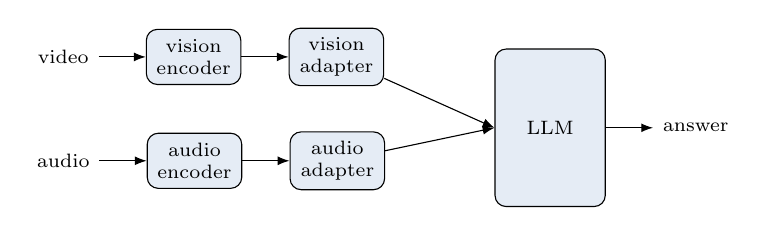
\begin{tikzpicture}[font=\scriptsize,>={Latex[length=1.5mm]},node distance=3.5mm and 6mm,
  enc/.style={draw,rounded corners,fill=frz!12,minimum width=12mm,minimum height=7mm,align=center},
  llm/.style={draw,rounded corners,fill=frz!12,minimum width=14mm,minimum height=20mm,align=center},
  io/.style={align=center}]
  \node[io] (vin) {video};
  \node[enc,right=of vin] (venc) {vision\\encoder};
  \node[enc,right=of venc] (vproj) {vision\\adapter};
  \node[io,below=9mm of vin] (ain) {audio};
  \node[enc,right=of ain] (aenc) {audio\\encoder};
  \node[enc,right=of aenc] (aproj) {audio\\adapter};
  \node[llm,right=14mm of vproj,yshift=-9mm] (llm) {LLM};
  \node[io,right=of llm] (ans) {answer};
  \draw[->] (vin)--(venc); \draw[->] (venc)--(vproj); \draw[->] (vproj)--(llm.west);
  \draw[->] (ain)--(aenc); \draw[->] (aenc)--(aproj); \draw[->] (aproj)--(llm.west);
  \draw[->] (llm.east)--(ans);
\end{tikzpicture}
\vspace{0.5em}
\begin{itemize}\footnotesize
\item Each modality is encoded into \textbf{tokens} (audio $\sim$25/s; video sampled at
\textbf{2\,fps} in all our Qwen3-Omni runs), projected by a small \emph{adapter} into the LLM's
embedding space, and concatenated with the question.
\item The LLM answers over the \textbf{mixed token sequence} --- text, audio and vision compete
for its attention.
\item Test beds: Qwen3-Omni (30B MoE), Qwen2.5-Omni (7B), VideoLLaMA2, MiniCPM-O 2.6.
\end{itemize}
\end{frame}

\begin{frame}{Problem statement: cross-modal hallucination}
\centering
\begin{tabular}{@{}c@{}}
\exrow{avh_a2v}{\textbf{audio $\to$ video} {\scriptsize(the sound makes it ``see'')}}{hear: harsh grinding, like a power tool. ``Is a power tool visible?'' --- no.}{``Yes''}{``No''} \\[2.5mm]
\exrow{avh_v2a}{\textbf{video $\to$ audio} {\scriptsize(the image makes it ``hear'')}}{see: a parrot on a shoulder; the clip is silent. ``Is the bird making sound?''}{``Yes''}{``No''}
\end{tabular}
\vfill
\footnotesize The model over-weights visual evidence relative to auditory evidence: it reports objects
implied by the audio (top) and sounds implied by the image (bottom).
\end{frame}

\begin{frame}{Related work: visual dominance in audio-visual LLMs}
\begin{itemize}\footnotesize\setlength\itemsep{3pt}
\item \textbf{AVHBench} (Sung-Bin et al., ICLR'25) establishes that cross-modal hallucination is
present in all evaluated audio-visual LLMs.
\item \textbf{CMM} (Leng et al., 2024) attributes the effect to over-reliance on unimodal priors,
with audio the most frequently overridden channel.
\item \textbf{Wen et al.\ (2026)} characterize it as a \emph{Clever Hans} effect: sound-related
questions are answered from visual priors rather than from the audio stream.
\item Existing mitigations --- contrastive decoding (MAD), modality-decoupled DPO (MoD-DPO) and
full-model re-alignment --- all modify or bypass the backbone; none operates on a frozen model.
\end{itemize}
\vfill
\centering
{\footnotesize Wen et al.'s audio interventions on \textbf{Qwen3-Omni} --- \emph{our} backbone (accuracy, \%):}\\[3pt]
\footnotesize
\begin{tabular}{l cc l}
\toprule
probe & original & intervened & intervention \\
\midrule
audio existence   & 95.1  & \textcolor{red!70!black}{\textbf{0.0}}  & \emph{Mute}: silence the track \\
temporal sync     & 100.0 & \textcolor{red!70!black}{\textbf{1.4}}  & \emph{Shift}: audio moved $\pm 2$\,s \\
sound consistency & 75.4  & \textcolor{red!70!black}{\textbf{37.3}} & \emph{Swap}: another clip's audio \\
\bottomrule
\end{tabular}\\[3pt]
{\scriptsize Reported values, arXiv:2605.16403, Tab.~1. Under muting, accuracy falls to zero:
responses remain consistent with the visual content.}
\end{frame}

\begin{frame}{Objective and contributions}
\begin{center}\large\itshape
Can audio grounding in a frozen audio-visual LLM be improved\\[2pt]
by training a parameter-efficient adapter alone?
\end{center}
\vspace{0.3em}
\begin{itemize}\footnotesize
\item[\textbf{C1}] A variational-bottleneck adapter ($<$0.5\% of parameters) that is exactly the
identity map at initialization.
\item[\textbf{C2}] An anchored preference objective that avoids the degenerate solution reached by
standard DPO, using two explicit constraints.
\item[\textbf{C3}] A query-conditioned (FiLM) variant, with attention-based evidence regarding its
mechanism.
\item[\textbf{C4}] An evaluation protocol with fixed decoding, held-out checkpoint selection, paired
significance testing, three capability controls and four backbones.
\item[\textbf{C5}] An extension to temporal alignment, including data construction, a benchmark and
a measured baseline.
\end{itemize}
\end{frame}

% ================================================================
% ================================================================

\begin{frame}{Evaluation benchmark: AVHBench}
\begin{columns}[T]
\begin{column}{0.5\textwidth}
\footnotesize
\setlength{\tabcolsep}{4pt}
\begin{tabular}{@{}lrrr@{}}
\toprule
Judgment task & QnA & yes & no \\
\midrule
A$\to$V (audio$\to$video) & 1,136 & 568 & 568 \\
V$\to$A (video$\to$audio) & 2,290 & 1,145 & 1,145 \\
A--V Matching             & 1,876 & 938 & 938 \\
\midrule
\textbf{Total}            & \textbf{5,302} & 2,651 & 2,651 \\
\bottomrule
\end{tabular}
\par\vspace{0.4em}
{\scriptsize 2,136 videos; yes/no labels are exactly balanced, so a constant response yields 50\%
accuracy.}
\end{column}
\begin{column}{0.5\textwidth}\scriptsize
\textbf{The three yes/no tasks}
\begin{itemize}
\item \textbf{A$\to$V}: whether a queried object is visible; the audible event induces false
positives.
\item \textbf{V$\to$A}: whether a queried sound is audible; the visible event induces false
positives. This is our primary measure of audio grounding.
\item \textbf{A--V Matching}: whether audio and video correspond; requires cross-modal
integration.
\end{itemize}
\end{column}
\end{columns}
\end{frame}

\begin{frame}{Capability benchmark: CMM}
\centering
{\footnotesize \textbf{1,200 samples $\times$ 2 probes $=$ 2,400 questions}: one \emph{present} object
(gold ``yes''), one \emph{absent} (gold ``no'') per sample.}
\vspace{0.5em}
\[
\mathbf{PA}=\frac{\#\,\text{correct ``yes''}}{\#\,\text{ground-truth ``yes''}}
\qquad\qquad
\mathbf{HR}=\frac{\#\,\text{correct ``no''}}{\#\,\text{ground-truth ``no''}}
\]
\begin{center}
\setbeamercolor{block body}{bg=red!6}
\begin{block}{Both metrics must be reported jointly}
\centering\footnotesize A model that answers ``no'' to every question attains HR $=$ 1.0 and PA $=$ 0.
Improvements in hallucination resistance must therefore be verified against a corresponding
degradation in perception accuracy.
\end{block}
\end{center}
\vfill
{\footnotesize This degenerate solution is not hypothetical: it is the outcome of our initial
training run (reported below).}
\end{frame}

\begin{frame}{Experimental protocol}
\begin{itemize}\footnotesize
\item \textbf{Frame rate} is fixed in code at 2\,fps for Qwen3-Omni (1\,fps for the 7B backbones),
identically for checkpoint selection and final evaluation. Below 2\,fps, Qwen3-Omni exhibits a
systematic bias toward affirmative answers.
\item \textbf{Prompt sensitivity is substantial.} Altering only the answer-format suffix changed one
score by $+11$ points (V$\to$A, $69.0 \to 80.3$) with identical weights. Prompts, suffix and decoding
parameters are therefore fixed and logged.
\item \textbf{Checkpoint selection} is performed on a validation half and results reported on the
disjoint remainder. The initially selected checkpoint did not survive this procedure.
\item \textbf{Significance testing} is paired (identical items for both models): McNemar's test with
bootstrap confidence intervals.
\item \textbf{Contamination check}: the intersection of training and benchmark clips is empty,
verified by script.
\end{itemize}
\vfill
\begin{center}
\setbeamercolor{block body}{bg=blue!6}
\begin{block}{}
\centering\footnotesize Reported accuracies are meaningful only relative to a fixed evaluation protocol.
\end{block}
\end{center}
\end{frame}

% ================================================================
% ================================================================

\begin{frame}{Background: the Variational Information Bottleneck}
{\footnotesize The information bottleneck (Tishby et al., 2000) seeks a compressed representation $Z$ of
the input $X$ that retains only the information predictive of the target $Y$.}
\vspace{-0.2em}
\[
\max_{q(z|x)}\ \underbrace{I(Z;Y)}_{\text{keep what predicts }Y}\ -\ \beta\,\underbrace{I(Z;X)}_{\text{forget the rest of }X}
\]
\vspace{-0.5em}
\begin{itemize}\footnotesize
\item Both mutual-information terms are intractable and are replaced by variational bounds (Alemi
et al., ICLR'17): the compression term is upper-bounded by
$\mathbb E_x\,\mathrm{KL}\!\big(q(z|x)\,\|\,\mathcal N(0,I)\big)$, referred to as the rate; the
relevance term reduces to the prediction loss.
\item The encoder is stochastic and trained by reparameterization,
$z=\mu(x)+\sigma(x)\odot\epsilon$ with $\epsilon\sim\mathcal N(0,I)$.
\item $\beta$ controls the compression-accuracy trade-off and corresponds to $\beta_{kl}$ in our
objective.
\end{itemize}
\end{frame}

\begin{frame}{Method: a variational bottleneck per modality stream}
\centering
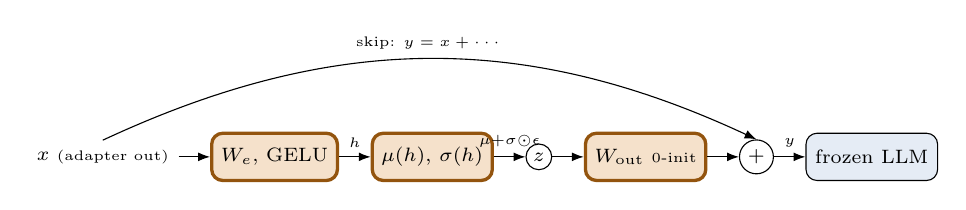
\begin{tikzpicture}[font=\scriptsize,>={Latex[length=1.5mm]},node distance=2mm and 4mm,
  trn/.style={draw,very thick,rounded corners,fill=trn!22,draw=trn!70!black,minimum height=6mm,align=center},
  frzs/.style={draw,rounded corners,fill=frz!12,minimum height=6mm,align=center},
  op/.style={draw,circle,inner sep=1.5pt},
  io/.style={align=center}]
  \node[io] (x) {$x$ {\tiny(adapter out)}};
  \node[trn,right=of x] (enc) {$W_e$, GELU};
  \node[trn,right=of enc] (ms) {$\mu(h),\,\sigma(h)$};
  \node[op,right=of ms] (z) {$z$};
  \node[trn,right=of z] (wout) {$W_{\text{out}}$ {\tiny 0-init}};
  \node[op,right=of wout] (add) {$+$};
  \node[frzs,right=of add] (llm) {frozen LLM};
  \draw[->] (x)--(enc); \draw[->] (enc)--node[above]{\tiny $h$}(ms);
  \draw[->] (ms)--node[above]{\tiny $\mu{+}\sigma{\odot}\epsilon$}(z);
  \draw[->] (z)--(wout); \draw[->] (wout)--(add);
  \draw[->] (add)--node[above]{\tiny $y$}(llm);
  \draw[->] (x.north) to[out=25,in=155] node[above,pos=0.5]{\tiny skip: $y=x+\cdots$} (add.north);
\end{tikzpicture}
\vspace{0.4em}
\[ z=\mu(x)+\sigma(x)\odot\epsilon \qquad y = x + W_{\text{out}}\,z \qquad W_{\text{out}}\stackrel{\text{init}}{=}0 \]
\begin{itemize}\footnotesize
\item Zero-initialization of $W_{\text{out}}$ gives $y=x$ at initialization: attaching the module
leaves the model's behaviour unchanged until training begins.
\item A bypass flag recovers the frozen backbone exactly, providing the DPO reference distribution
without instantiating a second model.
\item One module per modality (audio, vision), together $<$0.5\% of backbone parameters.
\end{itemize}
\end{frame}

\begin{frame}{Training data: constructed audio-visual conflicts}
\centering
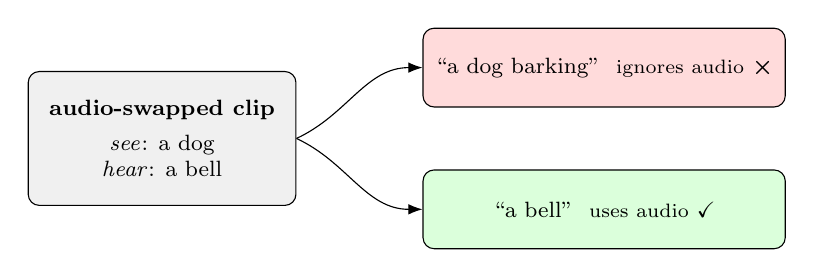
\begin{tikzpicture}[font=\footnotesize,>={Latex[length=1.8mm]},
  clip/.style={draw,rounded corners,fill=gray!12,align=center,minimum width=34mm,minimum height=17mm},
  good/.style={draw,rounded corners,fill=green!14,align=center,minimum width=46mm,minimum height=10mm},
  bad/.style={draw,rounded corners,fill=red!14,align=center,minimum width=46mm,minimum height=10mm}]
  \node[clip] (clip) {\textbf{audio-swapped clip}\\[1mm]\emph{see}: a dog\\\emph{hear}: a bell};
  \node[bad,right=16mm of clip,yshift=9mm] (bad) {``a dog barking'' \ {\scriptsize ignores audio} $\boldsymbol{\times}$};
  \node[good,right=16mm of clip,yshift=-9mm] (good) {``a bell'' \ {\scriptsize uses audio} $\boldsymbol{\checkmark}$};
  \draw[->] (clip.east) to[out=25,in=180] (bad.west);
  \draw[->] (clip.east) to[out=-25,in=180] (good.west);
\end{tikzpicture}
\vspace{0.4em}
\par
\exrow{as_flute}{\emph{see} flute, \textbf{hear (overlaid) train horn}}{``Which event do you hear?''}{``flute''}{``train horn''}
\vfill
\footnotesize Substituting a clip's audio track produces an instance in which the visible and audible
events disagree. Preferring the audio-consistent answer on such an instance requires use of the
audio stream.
\end{frame}

\begin{frame}{Failure mode of standard preference optimization}
\vspace{-0.2em}
\[
\mathcal L_{\text{DPO}}
=-\log\sigma^{\textcolor{trn}{*}}\Big(\beta^{\textcolor{trn}{**}}\big[\underbrace{(c_p-c_r)}_{\text{chosen: gain over base}}
-\underbrace{(r_p-r_r)}_{\text{rejected: gain over base}}\big]\Big)
\]
{\tiny \textcolor{trn}{$^{*}$}\,$\sigma=$ logistic sigmoid (\emph{not} the encoder's std-dev $\sigma(x)$).\quad
\textcolor{trn}{$^{**}$}\,$\beta=$ DPO temperature ($0.1$; \emph{not} the VIB rate $\beta_{kl}$).}
\vspace{2pt}
{\scriptsize $c,r$ $=$ log-probs of the chosen (heard) / rejected (seen) answer; subscript $p$ $=$
adapter on, $r$ $=$ adapter bypassed $=$ the frozen base --- our reference model, for free.}
\vspace{0.2em}
\begin{itemize}\footnotesize
\item Training with the standard DPO objective on these pairs reduces perception accuracy from
$0.95$ to $0.10$: the model converges to answering ``no'' for all inputs.
\item The objective constrains only the \emph{margin} between the two candidates. It is minimized
even when both probabilities decrease, provided the rejected candidate decreases faster; the
displaced mass accumulates on an unconstrained third response (\emph{likelihood displacement}).
\item Under CMM, this degenerate solution attains maximal hallucination resistance, which is why the
capability metric must be monitored jointly.
\end{itemize}
\vfill
\begin{center}
\setbeamercolor{block body}{bg=red!8}
\begin{block}{}
\centering\footnotesize A hallucination metric alone is not a sufficient training signal.
\end{block}
\end{center}
\end{frame}

\begin{frame}{Proposed objective: preference term with two constraints}
\vspace{-0.3em}
\begin{align*}
\mathcal L =\ & \underbrace{-\log\sigma(\beta[(c_p{-}c_r){-}(r_p{-}r_r)])}_{\text{\textbf{engine}: prefer the heard answer}}
 \;+\; \lambda_a\,\underbrace{\big({-}\log\sigma(\beta(c_p{-}c_r){-}\delta)\big)}_{\text{\textcolor{trn}{\textbf{rail 1}: chosen $\ge$ base $\Rightarrow$ PA}}} \\[2pt]
 &+\; \lambda_{kl}\,\underbrace{\mathrm{KL}\!\big(p_{\text{base}}\,\|\,p_\theta\big)}_{\text{\textcolor{trn}{\textbf{rail 2}: normal inputs unchanged $\Rightarrow$ HR}}}
 \;+\; \beta_{kl}\,\mathrm{KL}_{\text{VIB}}
\end{align*}
\vspace{-0.3em}
\begin{itemize}\footnotesize
\item The first constraint (an mDPO-style anchor) prevents the degenerate solution by requiring the
chosen response to retain at least its probability under the frozen backbone.
\item The second constraint penalizes divergence from the backbone on ordinary (non-substituted)
inputs, preserving capability.
\item Consequently, the uniform-``no'' solution violates both constraints, and the preference term
can only be reduced by using the audio stream.
\end{itemize}
\end{frame}

\begin{frame}{Query-conditioned variant (FiLM)}
\centering
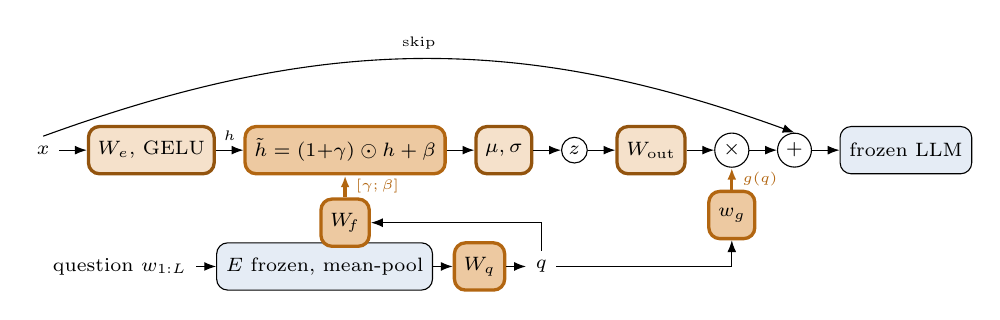
\begin{tikzpicture}[font=\scriptsize,>={Latex[length=1.5mm]},node distance=2mm and 3.5mm,
  trn/.style={draw,very thick,rounded corners,fill=trn!22,draw=trn!70!black,minimum height=6mm,align=center},
  new/.style={draw,very thick,rounded corners,fill=trn!40,draw=trn!85!black,minimum height=6mm,align=center},
  frzs/.style={draw,rounded corners,fill=frz!12,minimum height=6mm,align=center},
  op/.style={draw,circle,inner sep=1.5pt},
  io/.style={align=center}]
  \node[io] (x) {$x$};
  \node[trn,right=of x] (enc) {$W_e$, GELU};
  \node[new,right=of enc] (film) {$\tilde h=(1{+}\gamma)\odot h+\beta$};
  \node[trn,right=of film] (ms) {$\mu,\sigma$};
  \node[op,right=of ms] (z) {$z$};
  \node[trn,right=of z] (wout) {$W_{\text{out}}$};
  \node[op,right=of wout] (mult) {$\times$};
  \node[op,right=of mult] (add) {$+$};
  \node[frzs,right=of add] (llm) {frozen LLM};
  \draw[->] (x)--(enc); \draw[->] (enc)--node[above]{\tiny $h$}(film);
  \draw[->] (film)--(ms); \draw[->] (ms)--(z);
  \draw[->] (z)--(wout); \draw[->] (wout)--(mult); \draw[->] (mult)--(add);
  \draw[->] (add)--(llm);
  \draw[->] (x.north) to[out=20,in=160] node[above,pos=0.5]{\tiny skip} (add.north);
  \node[io,below=13mm of x,anchor=west] (w) {question $w_{1:L}$};
  \node[frzs,right=2.5mm of w] (embed) {$E$ frozen, mean-pool};
  \node[new,right=2.5mm of embed] (wq) {$W_q$};
  \node[io,right=2.5mm of wq] (qv) {$q$};
  \node[new] (wf) at ([yshift=-6mm]film.south) {$W_{\!f}$};
  \node[new] (wg) at ([yshift=-6mm]mult.south) {$w_g$};
  \draw[->] (w)--(embed); \draw[->] (embed)--(wq); \draw[->] (wq)--(qv);
  \draw[->] (qv.north) |- (wf.east);
  \draw[->] (qv.east) -| (wg.south);
  \draw[->,trn!85!black,very thick] (wf.north)--node[right]{\tiny $[\gamma;\beta]$}(film.south);
  \draw[->,trn!85!black,very thick] (wg.north)--node[right]{\tiny $g(q)$}(mult.south);
\end{tikzpicture}
\vspace{0.4em}
\begin{columns}[T]
\begin{column}{0.5\textwidth}
{\scriptsize \textcolor{trn}{\textbf{Main path}} {\normalfont(the plain VIB)}}
\begin{itemize}\scriptsize\setlength\itemsep{1pt}
\item $W_e$: encoder --- lifts token $x$ into hidden $h$
\item $\mu,\sigma$: latent heads --- $z=\mu+\sigma\odot\epsilon$
\item $W_{\text{out}}$: output, \textbf{zero-init}
\end{itemize}
\end{column}
\begin{column}{0.5\textwidth}
{\scriptsize \textcolor{trn}{\textbf{Question path}} {\normalfont(new in FiLM)}}
\begin{itemize}\scriptsize\setlength\itemsep{1pt}
\item $W_q$: pools frozen embeddings $E$ into $q$
\item $W_{\!f}$: $q\mapsto[\gamma;\beta]$ --- per-feature \textbf{scale} \& \textbf{shift}
\item $w_g$: $q\mapsto g(q)\!\in\!(0,1)$ --- \textbf{volume knob}
\end{itemize}
\end{column}
\end{columns}
\vspace{2pt}
{\scriptsize \textcolor{frz}{\textbf{Blue} $=$ frozen}. $\gamma,\beta$ are FiLM's scale/shift (Perez
et al., 2018), \emph{not} the loss's $\beta$ or $\beta_{kl}$. Zero-init $\Rightarrow$ identity at start.}
\end{frame}

\begin{frame}{Why query conditioning is required: a loss-floor argument}
{\footnotesize Consider one substituted clip (visible: dog; audible: bell) and two questions over
identical inputs: ``what do you hear?'' (target: bell) and ``what do you see?'' (target: dog). The
per-question loss is $-\log\sigma(m)$, giving $0.13$, $0.69$ and $2.13$ for margins
$m = +2$, $0$ and $-2$ respectively.}
\vspace{0.4em}
\centering
\renewcommand{\arraystretch}{1.15}
\footnotesize
\begin{tabular}{l l cc c}
\toprule
adapter & answers (HEAR / SEE) & HEAR loss & SEE loss & total \\
\midrule
can't read $q$, commits to ``bell'' & ``bell'' / ``bell'' & $0.13$ & $2.13$ & $2.26$ \\
can't read $q$, hedges 50/50        & --- & $0.69$ & $0.69$ & $\mathbf{1.39}$ (floor) \\
\textbf{reads $q$}                  & ``bell'' / ``dog''  & $0.13$ & $0.13$ & $\mathbf{0.26\to 0}$ \\
\bottomrule
\end{tabular}
\vspace{0.5em}
\par
{\footnotesize A query-independent adapter has a loss floor of $2\log 2 \approx 1.39$ per pair, whereas a
query-conditioned one attains zero. The data construction therefore makes query conditioning
necessary at the optimum. This is a property of the objective, not an empirical result.}
\end{frame}

% ================================================================
% ================================================================

\begin{frame}{Main results (Qwen3-Omni, full benchmarks)}
\centering
\renewcommand{\arraystretch}{1.2}
\footnotesize
\begin{tabular}{l cccc ccc}
\toprule
& \multicolumn{4}{c}{AVHBench (n$=$5302)} & \multicolumn{3}{c}{CMM (n$=$2400)} \\
\cmidrule(lr){2-5}\cmidrule(lr){6-8}
 & $A\!\to\!V$ & $V\!\to\!A$ & AV-m & overall & PA & HR & overall \\
\midrule
Gemini {\tiny(closed)} & 0.850 & 0.747 & 0.603 & 0.718 & 0.907 & 0.628 & 0.768 \\
GPT-4o {\tiny(closed)} & 0.846 & 0.510 & 0.501 & 0.579 & 0.359 & 0.892 & 0.626 \\
\midrule
frozen base            & \textbf{0.838} & 0.812 & 0.653 & 0.761 & \textbf{0.900} & 0.733 & 0.816 \\
$+$ cross-attention (step 60) & \textbf{0.850} & 0.805 & 0.696 & 0.776 & \multicolumn{3}{c}{\emph{CMM running}} \\
$+$ LoRA $r{=}16$ (step 90) & 0.828 & 0.835 & 0.709 & 0.789 & 0.896 & 0.724 & 0.810 \\
$+$ swap-DPO (step 60) & 0.837 & \textbf{0.838} & 0.766 & 0.812 & 0.890 & 0.743 & 0.816 \\
$+$ \textbf{FiLM} (step 160) & 0.822 & 0.827 & \textbf{0.808} & \textbf{0.819} & 0.894 & \textbf{0.746} & \textbf{0.820} \\
\bottomrule
\end{tabular}
\vfill
{\footnotesize All rows evaluated under the same fixed protocol; adapters selected on a validation
half. The proposed adapters improve overall accuracy by $+5.1$ and $+5.8$ points while preserving
capability (HR increases; PA decreases by at most one point). The improvement is concentrated in
A--V Matching ($0.653 \to 0.808$, $+15.5$). GPT-4o's combination of HR $0.892$ with PA $0.359$ is an
instance of the degenerate solution described above.}
\end{frame}

\begin{frame}{Statistical significance: paired analysis}
{\footnotesize Both models are evaluated on identical items, so only discordant pairs are
informative: of $N$ items, $b$ are answered correctly by the baseline alone and $c$ by the adapted
model alone.}
{\footnotesize
\[
\Delta=\tfrac{c-b}{N}\qquad
\text{95\% CI: }\Delta\pm 1.96\,\tfrac{\sqrt{(b+c)-(c-b)^2/N}}{N}\qquad
\text{McNemar: is }b/c\text{ a fair coin?}
\]}
\centering
\scriptsize
\renewcommand{\arraystretch}{1.1}
\begin{tabular}{l c c c}
\toprule
comparison (held-out) & $b$ / $c$ & $\Delta$ [95\% CI] & verdict \\
\midrule
base $\to$ swap-DPO & 152 / 411 & $+5.2$ [{+}4.3, {+}6.1] & real ($p<10^{-4}$) \\
base $\to$ FiLM     & 253 / 532 & $+5.6$ [{+}4.5, {+}6.7] & real ($p<10^{-4}$) \\
DPO $\to$ FiLM      & 204 / 224 & $+0.4$ [{-}0.4, {+}1.2] & tie; FiLM wins AV-m ($+3.7$, $p<10^{-4}$) \\
\bottomrule
\end{tabular}
\vspace{0.4em}
\par
{\footnotesize The discordant counts (411 versus 152) are inconsistent with an equal-probability
null. Results are from a single training seed; the intervals reflect item sampling only, not
variation across seeds.}
\end{frame}

\begin{frame}{Capability control I: audio understanding (MMAU, n$=$1000)}
\centering
\renewcommand{\arraystretch}{1.2}
\footnotesize
\begin{tabular}{l cccc}
\toprule
Qwen3-Omni & Sound & Music & Speech & Avg. \\
\midrule
frozen base    & \textbf{80.2} & \textbf{75.4} & \textbf{68.5} & \textbf{74.7} \\
$+$ swap-DPO   & 78.4 & 75.1 & 67.0 & 73.5 \\
$+$ FiLM       & 79.6 & 73.1 & 66.4 & 73.0 \\
\bottomrule
\end{tabular}
\par\vspace{0.3em}
{\scriptsize Measured, parse rate $0.94$ on all three rows.}
\vfill
\begin{itemize}\footnotesize
\item Both adapters incur a small cost ($-1.2$ for swap-DPO, $-1.7$ for FiLM). Both lie within the
$\pm2.8$-point interval at n$=$1000, but the sign is negative and is reported as such.
\item MMAU is out of distribution for this method: audio-only reasoning, without video or
hallucination-inducing constructions.
\item We conclude that learning which modality to rely upon does not transfer to audio
understanding in general.
\end{itemize}
\end{frame}

\begin{frame}{Capability control II: video understanding (Video-MME, n$=$900)}
\begin{columns}[T]
\begin{column}{0.5\textwidth}\footnotesize
\textbf{The benchmark}
\begin{itemize}\footnotesize
\item 900 YouTube videos $\times$ 3 MCQs; we run the \textbf{short} subset, \textbf{without
subtitles}, audio taken from the video itself.
\item Same pinned harness: 2\,fps, letter answers, same parser.
\end{itemize}
\end{column}
\begin{column}{0.5\textwidth}
\centering
\renewcommand{\arraystretch}{1.2}
\footnotesize
\begin{tabular}{l c c}
\toprule
Qwen3-Omni & acc & $\Delta$ \\
\midrule
frozen base  & \textbf{0.842} & --- \\
$+$ swap-DPO & 0.828 & $-1.4$ \\
$+$ FiLM     & 0.837 & $-0.6$ \\
\bottomrule
\end{tabular}
\end{column}
\end{columns}
\vfill
\begin{itemize}\footnotesize
\item The 95\% interval is $\pm2.4$ points; both differences fall inside it, indicating no
significant loss of general video-QA capability.
\item The ordering matches MMAU: FiLM preserves capability better than swap-DPO ($-0.6$ versus
$-1.4$).
\item Across the three controls, hallucination resistance (CMM) improves while audio and video
understanding show small, non-significant decreases. The improvement is specific to the training
distribution, and its cost elsewhere is quantified rather than assumed.
\end{itemize}
\end{frame}

% ================================================================
% ================================================================

\begin{frame}{Mechanism I: attention allocated to audio-visual tokens}
\begin{columns}[T]
\begin{column}{0.56\textwidth}
\centering
\figslot{attn_av.png}{\linewidth}\\[2pt]
{\scriptsize Share of the answer position's attention on audio/visual tokens, per clip
(box $=$ median/IQR). Eager attention; compare \textbf{within} a model only.}
\end{column}
\begin{column}{0.44\textwidth}\footnotesize
\begin{itemize}\footnotesize
\item Qwen3-Omni, base $\to$ swap-DPO: $5.4\% \to 5.7\%$ (unchanged within variation), indicating
grounding via re-encoding of the tokens rather than increased attention to them.
\item Qwen3-Omni, base $\to$ FiLM: $5.4\% \to 7.4\%$, a relative increase of $38\%$; this is the only
variant that increases attention to the audio-visual evidence.
\item Qwen2.5-Omni, base $\to$ swap-DPO: $7.9\% \to 8.1\%$.
\end{itemize}
\vspace{0.4em}
{\footnotesize Comparable benchmark improvements are therefore obtained through two distinct
mechanisms. The likelihood analysis (next slide) shows both variants increase audio dependence;
they differ in whether attention to the evidence also increases.}
\end{column}
\end{columns}
\end{frame}

\begin{frame}{Mechanism II: dependence of the answer on the audio}
\begin{columns}[T]
\begin{column}{0.54\textwidth}
\centering
\figslot{ll_shift.png}{\linewidth}\\[2pt]
{\scriptsize Log-likelihood of the gold answer under the true audio (teal) and under substituted
audio (magenta); KDE over 40 AVE clips, dashed lines are means.}
\end{column}
\begin{column}{0.46\textwidth}\footnotesize
{\footnotesize Substituting the audio and re-scoring the \emph{same} answer measures how much the
response depends on the audio stream. A model that ignores audio yields a shift near zero.}
\vspace{0.4em}
\centering
\scriptsize
\begin{tabular}{l c}
\toprule
Qwen3-Omni & shift \\
\midrule
frozen base    & $-0.515$ \\
$+$ swap-DPO   & $-1.698$ \\
$+$ FiLM       & $\mathbf{-1.848}$ \\
\bottomrule
\end{tabular}
\par\vspace{0.3em}
{\scriptsize Measured, n$=$40 pairs.}
\end{column}
\end{columns}
\vfill
\begin{itemize}\footnotesize
\item Both adapters increase audio dependence by a factor of roughly $3.3$--$3.6$ relative to the
frozen backbone; the difference between them is small.
\item Taken with the attention analysis, the two variants are separable: swap-DPO raises audio
dependence \emph{without} increasing attention to audio-visual tokens (re-encoding), whereas FiLM
raises both.
\end{itemize}
\end{frame}

\begin{frame}{Mechanism III: analysis of the learned parameters}
{\footnotesize Three measurements computed directly from the trained FiLM checkpoint, without inference:}
\vspace{0.3em}
\centering
\renewcommand{\arraystretch}{1.3}
\footnotesize
\begin{tabular}{l c l}
\toprule
probe & value & reading \\
\midrule
$\|W_{\text{out}}\|$ vs $\|W_e\|$ (spectral) & $\approx 1.0$ & the edit \textbf{rotates} features, does not amplify \\
FiLM gate $g(q)$ over the eval questions & never $<0.4$ & \textbf{modulation, not routing} --- it never switches off \\
FiLM modulation, vision vs audio & $\approx 4.5\times$ & the question steers mostly \textbf{through vision} \\
\bottomrule
\end{tabular}
\vfill
\begin{itemize}\footnotesize
\item An earlier version of this analysis reported that 59\% of the vision stream was rewritten with
the audio module inactive. Direct inspection of the parameters did not support that claim and it was
withdrawn.
\item The result is consistent with the attention analysis: the query-conditioned module acts in part
by re-weighting the visual contribution.
\end{itemize}
\end{frame}

\begin{frame}{Generalization across backbones}
\centering
\renewcommand{\arraystretch}{1.2}
\footnotesize
\begin{tabular}{l cc c l}
\toprule
backbone & base & $+$ adapter & $\Delta$ & attention to AV tokens \\
\midrule
Qwen3-Omni (30B)  & 0.761 & \textbf{0.819} & $+5.8$ & $5.4\% \to 7.4\%$ \\
Qwen2.5-Omni (7B) & 0.729 & 0.730 & $+0.1$ & $7.9\% \to 8.1\%$ \\
VideoLLaMA2 (7B)  & 0.707 & 0.684 & $\textcolor{red!70!black}{-2.3}$ & audio bolted on post-hoc \\
MiniCPM-O 2.6 (8B) & 0.744 & \emph{training} & --- & --- \\
\bottomrule
\end{tabular}
\par\vspace{0.4em}
{\scriptsize AVHBench overall accuracy, n$=$5302; identical data, objective, constraints and
selection procedure for every row.}
\vfill
\begin{itemize}\footnotesize
\item The improvement scales with the audio information already available in the frozen backbone:
substantial for Qwen3-Omni, negligible for Qwen2.5-Omni, and negative for VideoLLaMA2, whose audio
pathway was added post hoc.
\item This negative result bounds the method: a parameter-efficient adapter can make existing audio
information usable, but cannot supply audio competence the backbone lacks.
\end{itemize}
\end{frame}

\begin{frame}{A fourth backbone: MiniCPM-O 2.6 and harness sensitivity}
\centering
\renewcommand{\arraystretch}{1.2}
\footnotesize
\begin{tabular}{l cccc}
\toprule
MiniCPM-O 2.6, AVHBench & $A\!\to\!V$ & $V\!\to\!A$ & AV-m & overall \\
\midrule
base --- \emph{our} harness & 0.751 & 0.796 & 0.678 & \textbf{0.744} \\
base --- \emph{reported} {\scriptsize(arXiv:2603.03192)} & 0.834 & 0.745 & 0.543 & 0.693 \\
\bottomrule
\end{tabular}
\par\vspace{0.3em}
{\scriptsize Ours: n$=$5302, parse $1.00$. CMM (ours): PA $0.897$ / HR $\mathbf{0.578}$.}
\vfill
\begin{itemize}\footnotesize
\item Identical weights and benchmark differ by $5.1$ points between our measurement and the
published one, attributable to prompt, answer-format and frame-rate choices --- the protocol
sensitivity quantified earlier.
\item Accordingly, we compare relative improvements within a single protocol, not absolute
accuracies across publications.
\item MiniCPM-O's hallucination resistance (HR $0.578$, versus $0.733$ for Qwen3-Omni) indicates
substantially weaker audio grounding, and correspondingly more headroom for the adapter.
\end{itemize}
\end{frame}

\begin{frame}{Comparison with prior methods (relative improvements)}
\centering
\renewcommand{\arraystretch}{1.25}
\footnotesize
\begin{tabular}{l l c c l}
\toprule
backbone & method & base $\to$ trained & $\Delta$ & trains \\
\midrule
MiniCPM-O 2.6 & MoD-DPO++ {\scriptsize(reported)} & $0.693 \to 0.745$ & $+5.2$ & \textcolor{red!70!black}{full LLM} \\
Qwen2.5-Omni  & MoD-DPO++ {\scriptsize(reported)} & $0.708 \to 0.796$ & $+8.8$ & \textcolor{red!70!black}{full LLM} \\
Qwen2.5-Omni  & MAD {\scriptsize(reported)}       & $0.769 \to 0.816$ & $+4.7$ & \textcolor{frz}{decode-time} \\
\midrule
Qwen3-Omni    & \textbf{FiLM (ours)} & $0.761 \to 0.819$ & \textbf{+5.8} & \textcolor{trn}{\textbf{$<$0.5\% adapter, frozen}} \\
\bottomrule
\end{tabular}
\par\vspace{0.3em}
{\scriptsize Reported rows: arXiv:2603.03192 (Tab.~1) and arXiv:2601.21181 (Tab.~1), each on
\emph{their} backbone and harness --- hence deltas only.}
\vfill
\begin{itemize}\footnotesize
\item The proposed method ($+5.8$) falls between full fine-tuning ($+8.8$) and training-free
decoding ($+4.7$), while updating $<$0.5\% of parameters and remaining reversible.
\item On A--V Matching the improvement is $+15.5$ points, comparable to the $+15.0$ reported for
MoD-DPO.
\end{itemize}
\end{frame}

% ================================================================
% ================================================================

\begin{frame}{Temporal alignment: a remaining failure mode}
\begin{itemize}\footnotesize
\item Wen et al.\ report that Qwen3-Omni's temporal-synchronization accuracy falls from $100$ to
$1.4$ when the audio is displaced by $\pm2$\,s. We reproduce the effect under our own protocol:
\end{itemize}
\vspace{0.2em}
\centering
\renewcommand{\arraystretch}{1.2}
\footnotesize
\begin{tabular}{l c l}
\toprule
AVE-Shift (held-out, balanced $\Rightarrow$ chance $=0.50$) & acc & reading \\
\midrule
base --- synchronized vs shifted (n$=$200) & 0.495 & at chance \\
base --- lag vs lead (n$=$100)       & 0.500 & at chance \\
base --- $\pm2$\,s displacement only (n$=$200) & 0.495 & at chance \\
\midrule
$+$ shift-DPO (step 60) --- synchronized vs shifted & 0.515 & unchanged \\
$+$ shift-DPO (step 60) --- lag vs lead & 0.450 & unchanged \\
\bottomrule
\end{tabular}
\par\vspace{0.3em}
{\scriptsize Measured. All differences lie within the $\pm7$-point interval at these sample sizes.
The third row restricts the probe to $\pm2$\,s displacements --- four frames at 2\,fps, the largest
and most clearly resolvable offset.}
\vfill
\begin{itemize}\footnotesize
\item The same objective applies with a different intervention: displacing the audio by
$\Delta \in \pm\{0.5,1,2\}$\,s and preferring the correct synchronization judgment over the default
response. The preference term and both constraints are unchanged.
\item \textbf{This is not sufficient}, and the limitation is not the objective. Training on the
displaced data leaves accuracy at chance, and restricting the probe to the largest, most resolvable
displacement ($\pm2$\,s, four frames) does not help either: the frozen backbone is at chance there
as well.
\item We therefore conclude that \textbf{the backbone carries no usable temporal-alignment signal},
so there is nothing for an adapter to unlock. This is the same pattern observed for audio on
VideoLLaMA2: where the frozen representation lacks the information, a parameter-efficient adapter
cannot supply it.
\end{itemize}
\end{frame}

\begin{frame}{Proposed extension: temporal input features}
\centering\footnotesize
$\tilde x_t = \big[\,x_t;\ \sin(2\pi t/T),\ \cos(2\pi t/T)\,\big]
\qquad h = \mathrm{GELU}(W_e\,\tilde x_t)$
\vspace{0.3em}
\par
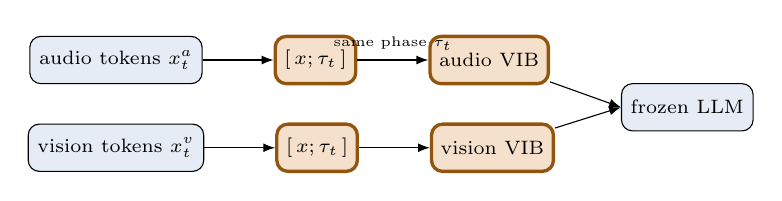
\begin{tikzpicture}[font=\scriptsize,>={Latex[length=1.5mm]},node distance=2mm and 4mm,
  trn/.style={draw,very thick,rounded corners,fill=trn!22,draw=trn!70!black,minimum height=6mm,align=center},
  frzs/.style={draw,rounded corners,fill=frz!12,minimum height=6mm,align=center}]
  \node[frzs] (a) {audio tokens $x^a_t$};
  \node[frzs,below=5mm of a] (v) {vision tokens $x^v_t$};
  \node[trn,right=9mm of a] (ca) {$[\,x;\tau_t\,]$};
  \node[trn,right=9mm of v] (cv) {$[\,x;\tau_t\,]$};
  \node[trn,right=9mm of ca] (ba) {audio VIB};
  \node[trn,right=9mm of cv] (bv) {vision VIB};
  \node[frzs,right=9mm of ba,yshift=-6mm] (llm) {frozen LLM};
  \draw[->] (a)--(ca); \draw[->] (v)--(cv);
  \draw[->] (ca)--node[above]{\tiny same phase $\tau_t$}(ba); \draw[->] (cv)--(bv);
  \draw[->] (ba)--(llm.west); \draw[->] (bv)--(llm.west);
\end{tikzpicture}
\vfill
\begin{itemize}\footnotesize
\item In the current formulation the bottleneck receives each token without positional information.
A shared phase $\tau_t$ across both streams makes misalignment representable: audio at time $t$ and a
frame at $t+\Delta$ then differ in their encodings.
\item At 2\,fps the frame interval is $0.5$\,s, which bounds the smallest resolvable displacement.
\item $W_{\text{out}}$ remains zero-initialized, preserving the identity property at initialization.
\item[] {\footnotesize\emph{Status: implemented and under training. Given that the backbone is at
chance even at $\pm2$\,s, we expect limited benefit; the run is retained as a controlled test of the
representability hypothesis rather than as an expected improvement.}}
\end{itemize}
\end{frame}

% ================================================================
% ================================================================

\begin{frame}{Ablation: placement of the bottleneck}
\centering
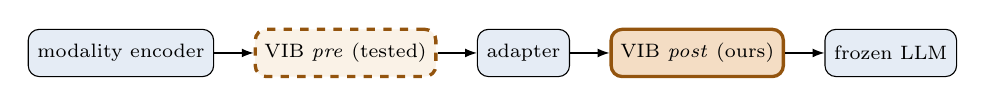
\begin{tikzpicture}[font=\scriptsize,>={Latex[length=1.5mm]},node distance=2mm and 5mm,
  frzs/.style={draw,rounded corners,fill=frz!12,minimum height=6mm,align=center},
  vibs/.style={draw,very thick,rounded corners,fill=trn!25,draw=trn!70!black,minimum height=6mm,align=center},
  vibd/.style={draw,very thick,dashed,rounded corners,fill=trn!10,draw=trn!70!black,minimum height=6mm,align=center}]
  \node[frzs] (enc) {modality encoder};
  \node[vibd,right=of enc] (pre) {VIB \emph{pre} (tested)};
  \node[frzs,right=of pre] (ad) {adapter};
  \node[vibs,right=of ad] (post) {VIB \emph{post} (ours)};
  \node[frzs,right=of post] (llm) {frozen LLM};
  \draw[->] (enc)--(pre); \draw[->] (pre)--(ad); \draw[->] (ad)--(post); \draw[->] (post)--(llm);
\end{tikzpicture}
\vspace{0.6em}
\begin{itemize}\footnotesize
\item The bottleneck is applied to the adapter's \emph{output} (the LLM embedding space). The
alternative is to apply it to the adapter's \emph{input} (raw encoder features).
\item The two placements produce comparable AVHBench accuracy; the choice is not decisive for
performance.
\item We retain the post-adapter placement because it uses a single attachment width (the LLM
hidden size) on all backbones, whereas the pre-adapter variant requires a distinct width per
modality and per backbone.
\item[] {\footnotesize\emph{The pre-adapter attachment is implemented (\texttt{--pre-adapter}); the
numerical results of the earlier comparison are not present in the current results directory and are
therefore not tabulated.}}
\end{itemize}
\end{frame}

\begin{frame}{Negative results}
\centering
\renewcommand{\arraystretch}{1.3}
\scriptsize
\resizebox{\linewidth}{!}{%
\begin{tabular}{l l l}
\toprule
tried & failure & lesson \\
\midrule
standard DPO on swap pairs & collapse to a constant response (PA $0.95\!\to\!0.10$) & motivated the two constraints \\
GRPO on low-difficulty items & zero advantage on $\sim$2/3 of steps & unanimous rewards provide no gradient \\
query-conditioned gate $g(q)$ & remained $>0.4$ throughout & modulation is preferred to routing \\
``59\% of vision rewritten'' & not supported by parameter inspection & claim withdrawn \\
LoRA at identical attach points & $+2.8$ versus $+5.1$; HR below base & the residual form matters, not capacity \\
\bottomrule
\end{tabular}}
\vfill
{\footnotesize Several of these results informed the final design and are reported for completeness.}
\end{frame}

\begin{frame}{Reproducibility}
\begin{columns}[T]
\begin{column}{0.52\textwidth}
\textbf{What exists}
\begin{itemize}\footnotesize
\item four model wrappers, five benchmark runners, four training variants, two baselines, three
analysis probes
\item approximately 10k lines of code, 23 cluster job scripts, seven test suites
\item each table and figure is produced by a single script
\end{itemize}
\end{column}
\begin{column}{0.48\textwidth}
\textbf{What is pinned}
\begin{itemize}\footnotesize
\item frame rate (2\,fps), prompts, answer format and decoding parameters
\item checkpoint selection on a disjoint validation half
\item per-item predictions are stored, so paired tests can be recomputed
\end{itemize}
\end{column}
\end{columns}
\vfill
\begin{center}
\setbeamercolor{block body}{bg=blue!6}
\begin{block}{}
\centering\footnotesize Every value reported here is either measured under our protocol (with the source
file identified in the document source) or taken from a cited publication.
\end{block}
\end{center}
\end{frame}

\begin{frame}{Conclusion}
\begin{itemize}
\item \textbf{Problem.} Frozen audio-visual LLMs over-weight visual evidence; on temporal
alignment they perform at chance ($0.495$, measured).
\item \textbf{Method.} A zero-initialized variational adapter ($<$0.5\% of parameters) trained with
an anchored preference objective on constructed audio-visual conflicts, plus a query-conditioned
variant.
\item \textbf{Results.} $+5.1$ and $+5.8$ AVHBench points ($p<10^{-4}$, paired), with hallucination
resistance preserved and non-significant differences on MMAU and Video-MME.
\item \textbf{Mechanism.} The query-conditioned variant is the only one that increases attention to
audio-visual tokens ($5.4\% \to 7.4\%$); the unconditional variant improves accuracy by re-encoding.
\item \textbf{Limitations.} The improvement requires a backbone with usable audio representations
(no effect on VideoLLaMA2), and out-of-distribution audio reasoning shows a small cost.
\item \textbf{Future work.} Extending the same objective to temporal alignment.
\end{itemize}
\vfill
\begin{center}
\setbeamercolor{block body}{bg=blue!6}
\begin{block}{}
\centering\footnotesize A parameter-efficient adapter improves audio grounding in a frozen audio-visual
LLM, and the improvement is supported by mechanistic evidence in addition to benchmark accuracy.
\end{block}
\end{center}
\end{frame}

\begin{frame}{Thank you}
\begin{columns}[T]
\begin{column}{0.58\textwidth}
\textbf{Acknowledgements}
\begin{itemize}\footnotesize
\item Qiu Yue and the AIST CVRT team.
\item Computation carried out on the ABCI cluster (group \texttt{gae50891}).
\end{itemize}
\vspace{0.6em}
\textbf{Experiments in progress}
\begin{itemize}\footnotesize
\item video-substitution and temporal-displacement training variants
\item MiniCPM-O adapter training and evaluation
\end{itemize}
\end{column}
\begin{column}{0.42\textwidth}
\centering
\vspace{0.4em}
{\Large Questions?}\\[1.2em]
{\footnotesize \color{gray} Souleiman Sbai\\[2pt]
\texttt{souleiman.sbai@polytechnique.edu}\\[1pt] \texttt{+33 6 20 94 64 63}}
\end{column}
\end{columns}
\end{frame}

\end{document}
